We consider the following setting: there are $\green{T}$ time steps\marginnote{$\green{T}$ might even be infinite.}, and $\ns$ ``experts'' $\Algo_1,\dots, \Algo_\ns$: at each time step $t$, the algorithm $\Algo$ 
\begin{itemize}
    \item receives advice $v_{1,t},\dots, v_{\ns,t}\in \bool$ from the experts, where $v_{i,t}$ comes from $\Algo_i$;
    \item outputs a prediction $\widehat{u}_t\in \bool$;
    \item after the prediction is made, gets the ground truth $u_t\in\{0,1\}$, and pays cost
    \[
    \purple{c}_t \eqdef \indicSet{\widehat{u}_t\neq u_t}
    \]
\end{itemize}
There is no assumption on the true values: they could be correlated, independent, adversarial. There is no assumption on the experts either: they could collude, be randomised, be adversarial, be omniscient. And there is no constraint on the algorithm itself: it can use as much memory as needed, be computationally inefficient, etc. But it \emph{cannot see the future}: all the information it has, at each time step $t$, is what happened in previous time steps, along with the current advice $v_{1,t},\dots, v_{\ns,t}$ from the experts.

\begin{framed}
    How to minimise the total cost $\purple{C}(\green{T})=\sum_{t=1}^{\green{T}} \purple{c}_t$?
\end{framed}

First, what does it even mean to minimise the total cost? How to formulate what this means? Can we get total cost, say, $\purple{C}(\green{T}) = o(\green{T})$? $\purple{C}(\green{T}) = O(\log \green{T})$?

\paragraph{Some bad news.}
\begin{fact}
    For any deterministic algorithm $\Algo$, and for any set of $\ns$ experts, there is a sequence $u_1,\dots, u_{\green{T}}$ such that $\Algo$ must have cost $\purple{C}(\green{T}) = \green{T}$.
\end{fact}
\begin{proof}
    $\widehat{u}_t$ is fully determined by the past, and the advice received: set $u_t = 1-\widehat{u}_t$.
\end{proof}

Of course, it is for \emph{deterministic} algorithms, these weaklings. Unfortunately, randomised algorithms do not do much better:
\begin{fact}
    For any algorithm $\Algo$, and for any set of $\ns$ experts, there is a distribution over sequences $u_1,\dots, u_{\green{T}}$ such that $\Algo$ must have expected cost $\expect{\purple{C}(\green{T})} \geq \frac{\green{T}}{2}$.
\end{fact}
\begin{proof}
    Uniformly random sequence.
\end{proof}

\paragraph{Changing the goal.} 
In view of this seriously underwhelming state of affairs, we need to reconsider either the \emph{setting}, or the \emph{objective}. We will do the second: in particular, one observation is that while in these bad examples the algorithm $\Algo$ does very poorly, \emph{so do all the $\ns$ experts}. This suggests that the right thing to try to achieve is not a small \emph{absolute} error, but an small error compared to that of \emph{the best expert in hindsight}. Namely, after $T$ steps, let 
\[
    \purple{C^\ast}(\green{T})= \min_{1\leq i\leq \ns }\sum_{t=1}^{\green{T}} \indicSet{v_{i,t}\neq u_t}
\]
denote the minimum cost achieved by the best of the $\ns$ experts.
\begin{framed}
    How to minimise the cost $\purple{C}(\green{T})$ compared to $\purple{C^\ast}(\green{T})$?
\end{framed}
%Let us call this quantity $\Delta(\green{T})$ the \emph{regret} of the algorithm.

\paragraph{Still some bad news.}
Even then, we cannot do \emph{arbitrarily} close to $\purple{C^\ast}(\green{T})$, at least not with a deterministic algorithm: a multiplicative factor at least $2$ is necessary.
\begin{fact}
    \label{theo:lb:deterministic}
    For any deterministic algorithm $\Algo$, and for any set of $\ns$ experts, there is a sequence $u_1,\dots, u_{\green{T}}$ such that $\Algo$ must have regret $\purple{C}(\green{T}) = \green{T}$, but $\purple{C^\ast}(\green{T}) \leq \frac{\green{T}}{2}$.
\end{fact}
\begin{proof}
    In the tutorial. %% Theorem 1.4 of [DH]
\end{proof}
\paragraph{Warmup: one perfect expert}
But there is some good news, too! Imagine one of the $\ns$ experts makes \emph{no mistakes.} Of course, we do not know which one in advance: yet, we \emph{can} leverage this.
\begin{theorem}\marginnote{Consistent Expert}
There is a (deterministic) algorithm (\cref{algo:consistent}) such that, if one of the $\ns$ experts makes \emph{zero} mistakes, \ie $\purple{C^\ast}(\green{T}) = 0$, then 
\[
\purple{C}(\green{T}) \leq \ns-1\,.
\]
Moreover, this holds even when $\green{T}=\infty$.
\end{theorem}
\begin{algorithm}[htbp]
\begin{algorithmic}[1]
    \State Set $S\gets [\ns]$
    \ForAll{$1\leq t\leq \green{T}$}
        \State Receive $v_{1,t},\dots, v_{\ns,t}$
        \If{$|S| \geq 1$}
            \State Pick any $i\in S$ \Comment{Lexicographically, for instance} \label{algo:experts:consistent:pick1}
            \State Choose $\widehat{u}_t \gets v_{i,t}$
        \Else 
            \State Choose $\widehat{u}_t \gets 0$ \Comment{Arbitrary}
        \EndIf
        \State Receive $u_t$ \Comment{Observe the truth}
        \State $S \gets S \setminus \{i \in S: v_{i,t} \neq u_t\}$ \Comment{Remove all mistaken experts}
    \EndFor
\end{algorithmic}
\caption{Consistent Expert algorithm}\label{algo:consistent}
\end{algorithm}
\begin{proof}
    The proof uses what is known as a \emph{potential argument}, where we define\marginnote{Potential argument} a suitable quantity $\Phi$ such that (1)~initially, $\Phi \leq \Phi_0$, (2)~at the end, $\Phi \geq \Phi_\infty$, and (3)~every time a ``bad event'' happens, $\Phi$ decreases by a quantifiable amount (typically, either decreases by at least some quantity $\Delta>0$ or by a constant factor $\gamma > 1$). By putting all 3 together, we are able to argue that the number of ``bad events'' is bounded by some values (which depends on $\Phi_0, \Phi_\infty$, and $\Delta$ or $\gamma$).

    Here, our potential function $\Phi$ is simply $\Phi=|S_t|$, where $S_t$ is the set $S$ at the end of step $1\leq t \leq \green{T}$. We have, at the beginning, $\Phi=\Phi_0 \eqdef |[\ns]| = \ns$; and, at the end, since by assumption at least \emph{one} expert never makes any mistake and thus is never removed from $S$, $\Phi_\infty = |S_{\green{T}}| \geq  1$.

    The ``bad event'' is when the algorithm makes a mistake: if this happens at time $t$, it is because the expert chosen from $S=S_{t-1}$ in Step~\ref{algo:experts:consistent:pick1} was wrong, and so it will be removed from $S_{t-1}$: which means $|S_t|$ decreases by (at least) $\Delta=1$: $\Phi_{t} \leq \Phi_{t-1} - \Delta$.

    Putting it all together, if we make $\purple{C}$ mistakes then our potential $\Phi$ decreases by at least $\Delta \cdot \purple{C}$: 
    \[
    1\leq \Phi_\infty \leq \Phi_0 - \Delta \cdot \purple{C} = \ns - 1\cdot \purple{C}
    \]
    and so $\purple{C} \leq \ns -1$.
\end{proof}

However, we can do even better! The main insight in the previous algorithm was that, every time we made a mistake, we could remove at least \emph{one} expert from the pool $S$. What if we could remove at least \emph{a constant fraction} of them?
\begin{theorem}\marginnote{Halving Algorithm}
    \label{theo:halving}
There is a (deterministic) algorithm (\cref{algo:halving}) such that, if one of the $\ns$ experts makes \emph{zero} mistakes, \ie $\purple{C^\ast}(\green{T}) = 0$, then 
\[
\purple{C}(\green{T}) \leq \log_2 \ns\,.
\]
Moreover, this holds even when $\green{T}=\infty$.
\end{theorem}
(As a side note: there is ``no free lunch.'' If we create $2^{\green{T}}$ \emph{fake experts}, one for each possible sequence $u_1,\dots,u_{\green{T}}$, then of course one of them will make no mistake: but then, the RHS in the theorem above becomes $\green{T}$.)
\begin{algorithm}[htbp]
\begin{algorithmic}
    \State Set $S\gets [\ns]$
    \ForAll{$1\leq t\leq \green{T}$}
        \State Receive $v_{1,t},\dots, v_{\ns,t}$
        \If{$|S| \geq 1$}
            \State Choose $\widehat{u}_t \gets \operatorname{maj}_{i\in S }v_{i,t}$ \Comment{Take the majority advice}
        \Else 
            \State Choose $\widehat{u}_t \gets 0$ \Comment{Arbitrary}
        \EndIf
        \State Receive $u_t$ \Comment{Observe the truth}
        \State $S \gets S \setminus \{i \in S: v_{i,t} \neq u_t\}$ \Comment{Remove all mistaken experts} \label{alg:experts:halving:step}
    \EndFor
\end{algorithmic}
\caption{Halving algorithm}\label{algo:halving}
\end{algorithm}
\begin{proof}
    Again, we will use a potential function argument, taking $\Phi=|S_t|$ as our potential. As before, $\Phi_0 = \ns$, while $\Phi_\infty = |S_{\green{T}}| \geq  1$; the main difference is that, each time we make a mistake, we know that this is before \emph{at least half} of the current experts in $S_t$ were wrong (as we took a majority vote among them), and so every time we make a mistake (``bad event'') Step~\ref{alg:experts:halving:step} will remove at least a $\gamma = 1/2$ fraction of $\Phi$.\footnote{The algorithm might also decrease $S$ in Step~\ref{alg:experts:halving:step}, and so $\Phi$, when we do \emph{not} make a mistake: but we cannot prove anything about this, when or if it happens, and by how much.}

    As a result, if we make $\purple{C}$ mistakes then our potential $\Phi$ decreases by at least $\Paren{1-\gamma}^{\purple{C}}$: 
    \[
    1\leq \Phi_\infty \leq \Phi_0 \cdot \Paren{1-\gamma}^{\purple{C}} = \frac{\ns}{2^{\purple{C}}}
    \]
    and so $\purple{C} \leq \log_2 \ns$.
\end{proof}

The theorem above is very good if at least one of the $\ns$ experts is perfect. Unfortunately, this is very seldom the case: what can we say when all experts make some mistake, sometimes? Can we do anything?

\paragraph{Making this robust.}
Here is an alternative view of the Halving algorithm:
\begin{itemize}
    \item We start with $\ns$ weights, $w_1=\dots = w_\ns = 1$.
    \item We answer according to the \emph{weighted majority} \[
    \operatorname{maj}_{1\leq i\leq \ns} w_i v_{i,t}
    \]
    \item If an expert $i$ is wrong at some step $t$, then their weight is set to $0$: $w_i \gets \red{0}\cdot w_i$.
\end{itemize}
This may sound a little extreme: ``one strike and you're out.'' Instead of setting a weight to \emph{zero} when a mistake is made, we could, instead, \emph{decrease} it.

\begin{algorithm}[htbp]
\begin{algorithmic}[1]
    \State Set $w_1,\dots, w_\ns \gets  1$
    \ForAll{$1\leq t\leq \green{T}$}
        \State Receive $v_{1,t},\dots, v_{\ns,t}$
        \State Choose $\widehat{u}_t \gets \sign\Paren{ \sum_{i=1}^\ns w_i v_{i,t} \geq \frac{1}{2}\sum_{i=1}^\ns w_i}$ \Comment{Weighted majority}
        \State Receive $u_t$ \Comment{Observe the truth}
        \ForAll{$1\leq i\leq \ns$} \Comment{Penalise all mistaken experts}
        \State $w_i \gets \begin{cases}
            \frac{1}{2} w_i & \text{ if } v_{i,t} \neq u_t\\
            w_i & \text{ otherwise.}
            \end{cases}$~\label{alg:experts:mwu:halving:step}
        \EndFor
    \EndFor
\end{algorithmic}
\caption{(Basic) Multiplicative Weights Updates algorithm}\label{algo:wmu:1}
\end{algorithm}

\begin{theorem}\marginnote{Basic MWU Algorithm}
    \label{theo:basic:mwu}
There is a (deterministic) algorithm (\cref{algo:wmu:1}) such that 
\[
\purple{C}(\green{T}) \leq \frac{\purple{C^\ast}(\green{T}) + \log_2 \ns}{\log_2 \frac{4}{3}} \leq 2.41\Paren{\purple{C^\ast}(\green{T})+\log_2 \ns}\,.
\]
Moreover, this holds even when $\green{T}=\infty$.
\end{theorem}
\begin{proof}
    Again (again), we will use a potential function argument, but this time defining our potential function $\Phi$ as
    \[
        \Phi= W_t
    \]
    where $W_t = \sum_{i=1}^\ns w_{i,t}$ (introducing new notation to get the dependence on $t$) is the sum of the weights of the $\ns$ experts at the beginning of time $t$.

    We get $\Phi_0 = \ns$, but now we can no longer bound $\Phi_\infty$ by $1$; however, we know that, by definition, there will be at least one expert who makes only $\purple{C^\ast}$ mistakes in total. That expert will be penalised and see its weight scaled by $1/2$ $\purple{C^\ast}$ times, and so at the end will still have weight $1/2^{\purple{C^\ast}}$. But the total weight at the end is at least the weight of that one expert, and so
    \[
        \Phi_\infty \geq \frac{1}{2^{\purple{C^\ast}}}\,.
    \]
    Moreover, since we are taking a (weighted) majority we know, as in the proof of~\cref{theo:halving}, that each time we make a mistake \emph{at least half of the total weight} of the experts was on wrong experts, and so every time we make a mistake (``bad event'') Step~\ref{alg:experts:mwu:halving:step} will remove at least a $1/2$ fraction of the ``wrong experts'' weight: call this $W_t^{\rm wrong}$. But our potential function is the \emph{total} weight, so \emph{what decrease does that imply for $W_t$?} 

    Writing 
    \[
    W_t = \underbrace{W_t^{\rm wrong}}_{\substack{\text{weight on experts wrong}\\\text{at time }t}} + \underbrace{(W_t-W_t^{\rm wrong})}_{\substack{\text{weight on experts correct}\\\text{at time }t}}
    \]
    we get that, if a mistake is made by the algorithm at time $t$, then
    \begin{align*}
    W_{t+1}
    &= \orange{\frac{1}{2}}\cdot W_t^{\rm wrong} + (W_t-W_t^{\rm wrong}) \\
    &= W_t - \frac{1}{2}W_t^{\rm wrong} \\
    &\leq W_t - \frac{1}{2}\cdot \frac{1}{2}W_t \tag{The majority was wrong: $W_t^{\rm wrong} \geq \frac{1}{2}W_t$} \\
    &= \frac{3}{4}W_t
    \end{align*}
    That is, at every mistake Step~\ref{alg:experts:halving:step} will remove at least a $\gamma = 1/4$ fraction of the total weight.
    As a result, if we make $\purple{C}$ mistakes then our potential $\Phi$ decreases by at least $\Paren{1-\gamma}^{\purple{C}}$: 
    \[
    \frac{1}{2^{\purple{C^\ast}}}\leq \Phi_\infty \leq \Phi_0 \cdot \Paren{1-\gamma}^{\purple{C}} = \Paren{\frac{3}{4}}^{\purple{C}}\cdot \ns
    \]
    and so $\purple{C} \leq \frac{\purple{C^\ast} + \log_2 \ns}{\log_2(4/3)}$.
\end{proof}

Now, there is nothing too special about $1/2$, except that it is a convenient number. We could instead keep it a ``penalty parameter'' $\orange{\beta}\in(0,1)$. This gives the following variant of the MWU:

\begin{algorithm}[htbp]
\begin{algorithmic}[1]
    \Require Penalty parameter $\orange{\beta}\in(0,1)$
    \State Set $w_1,\dots, w_\ns \gets  1$
    \ForAll{$1\leq t\leq \green{T}$}
        \State Receive $v_{1,t},\dots, v_{\ns,t}$
        \State Choose $\widehat{u}_t \gets \sign\Paren{ \sum_{i=1}^\ns w_i v_{i,t} \geq \frac{1}{2}\sum_{i=1}^\ns w_i}$ \Comment{Weighted majority}
        \State Receive $u_t$ \Comment{Observe the truth}
        \ForAll{$1\leq i\leq \ns$} \Comment{Penalise all mistaken experts}
        \State $w_i \gets \begin{cases}
            \orange{\beta} w_i & \text{ if } v_{i,t} \neq u_t\\
            w_i & \text{ otherwise.}
            \end{cases}$
        \EndFor
    \EndFor
\end{algorithmic}
\caption{Multiplicative Weights Updates algorithm}\label{algo:wmu:2}
\end{algorithm}

\begin{theorem}\marginnote{MWU Algorithm}
\label{theo:wmu}
There is a (deterministic) algorithm (\cref{algo:wmu:2}) such that 
\[
\purple{C}(\green{T}) \leq \frac{\purple{C^\ast}(\green{T})\log_2(1/\orange{\beta}) + \log_2 \ns}{\log_2 \frac{2}{1+\orange{\beta}}}\,.
\]
Moreover, this holds even when $\green{T}=\infty$.
\end{theorem}
\begin{proof}
    Same proof as~\cref{theo:basic:mwu}, but replacing $1/2$ by $\orange{\beta}$ in the appropriate locations.\marginnote{Good practice: go through the details!}
\end{proof}
In this sense, $\orange{\beta}$ lets us trade-off robustness ($\orange{\beta}\to 1$) for accuracy ($\orange{\beta}\to 0$). One can check that for $\orange{\beta}=1/2$, we get back the guarantees of~\cref{theo:basic:mwu}\marginnote{Check it!}, and that
\begin{itemize}
    \item When $\orange{\beta} \to 0$ and , we get
    \[
        \frac{\purple{C^\ast}(\green{T})\log_2(1/\orange{\beta}) + \log_2 \ns}{\log_2 \frac{2}{1+\orange{\beta}}} \operatorname*{\sim}_{\orange{\beta}\to 0^+} \log_2 \frac{1}{\orange{\beta}}\cdot \purple{C^\ast}(\green{T}) + \log_2\ns 
    \]
    retrieving the guarantees of~\cref{theo:halving} when $\purple{C^\ast}(\green{T})=0$;
    \item if $\orange{\beta} = 1-\orange{\eps}$ with $\orange{\eps} \to 0^+$, then
    \[
        \frac{\purple{C^\ast}(\green{T})\log_2(1/\orange{\beta}) + \log_2 \ns}{\log_2 \frac{2}{1+\orange{\beta}}} \operatorname*{\sim}_{\orange{\eps}\to 0^+} 2\cdot \purple{C^\ast}(\green{T}) + \frac{2}{\orange{\eps}}\ln \ns 
    \]
    much better in terms of dependence\footnote{Recall that a factor $2$ there is optimal for deterministic algorithms, by~\cref{theo:lb:deterministic}.} on $\purple{C^\ast}$, but \emph{much} worse with respect to the additive $\log_2\ns$.
\end{itemize}

\paragraph{But can we do better?} Our impossibility result (lower bound) from~\cref{theo:lb:deterministic} applies to deterministic algorithms. The MWU algorithm, which achieves this bound, is deterministic. If we allow \emph{randomisation} (and relax our goal a little to allow \emph{expected} error, can we circumvent this lower bound?

The answer is (of course?) yes. What is even better, this leads to a simple and very natural algorithm! 

Here again, the crucial observation is that~\cref{algo:wmu:2} takes a ``hard'' majority: the algorithm will predict the same thing if the weighted majority is $50.1\%$ or if it is $100\%$. This sounds a little silly: if our weighting of experts predicts essentially a coin toss, maybe we should not treat it too confidently?\marginnote{Maybe we should\dots toss a coin?}

\begin{algorithm}[htbp]
\begin{algorithmic}[1]
    \Require Penalty parameter $\orange{\beta}\in(0,1)$
    \State Set $w_1,\dots, w_\ns \gets  1$
    \ForAll{$1\leq t\leq \green{T}$}
        \State Receive $v_{1,t},\dots, v_{\ns,t}$
        \State Draw $\blue{I}\in[\ns]$ according to the weights:
        \[
            \probaOf{\blue{I} = i} = \frac{w_i}{\sum_{i=1}^\ns w_i}, \qquad i\in[\ns]
        \]
        \State Choose $\widehat{u}_t \gets v_{\blue{I},t}$ \Comment{One expert gets the vote}
        \State Receive $u_t$ \Comment{Observe the truth}
        \ForAll{$1\leq i\leq \ns$} \Comment{Penalise all mistaken experts}
        \State $w_i \gets \begin{cases}
            \orange{\beta} w_i & \text{ if } v_{i,t} \neq u_t\\
            w_i & \text{ otherwise.}
            \end{cases}$ \label{alg:experts:randmwu:beta}
        \EndFor
    \EndFor
\end{algorithmic}
\caption{Randomised Multiplicative Weights Updates algorithm}\label{algo:wmu:3}
\end{algorithm}
Observe that, in our binary setting where $u_t\in\bool$, what the algorithm does is equivalent to computing 
\[
    \tilde{p}_t \eqdef \sum_{i=1}^\ns \frac{w_i}{\sum_{j=1}^\ns w_j}\indic{v_{i,t}=1}
\]
and setting $\widehat{u}_t\sim \bernoulli{\tilde{p}_t}$. But phrasing it this way makes it easier to generalise to more complicated predictions than binary, and also can be more efficient to implement.\marginnote{Can you see why?}

\begin{theorem}\marginnote{MWU Algorithm}
    \label{theo:wmu:rand}
There is a (randomised) algorithm (\cref{algo:wmu:3}) such that 
\[
\expect{\purple{C}(\green{T})} \leq \frac{\purple{C^\ast}(\green{T})\ln(1/\orange{\beta}) + \ln \ns}{1-\orange{\beta}}\,.
\]
Moreover, this holds even when $\green{T}=\infty$.
\end{theorem}
\begin{proof}
    Denote by $F_t$ the fraction of the total weight that is on ``wrong experts'' at time step $t$; that is, with the notation of the proof of~\cref{theo:basic:mwu}, 
    \[
    F_t = \frac{W_t^{\rm wrong}}{W_t} \in [0,1], \qquad 1\leq t\leq \green{T}
    \]
    Since we are choosing which decision to make by sampling an expert according to the weights, the probability to make a mistake at time $t$ is exactly $F_t$; and so, by linearity of expectation,
    \begin{equation}
        \label{eq:experts:randmwu:expected}
    \expect{\purple{C}(\green{T})}
    = \sum_{t=1}^{\green{T}} F_t\,.
    \end{equation}
    Following as in the previous proofs a potential argument, we again choose as potential function $\Phi$ the total weight of the experts:
    \[
        \Phi_t \eqdef W_t = \sum_{i=1}^\ns w_{i,t}\,.
    \]
    We again have $\Phi_0 = \ns$, and $\Phi_\infty \geq \orange{\beta}^{\purple{C^\ast}}$ (the best expert makes only $\purple{C^\ast}$ mistakes, and so its weight at the end is $\orange{\beta}^{\purple{C^\ast}}$). Now, Step~\ref{alg:experts:randmwu:beta} penalises the wrong experts at every step: in the previous theorems, we only kept track of this when our algorithm made a mistake, since this is all we had a handle on\footnote{Namely, all we could say is that ``at least half of the weight was on wrong experts'' \emph{when we made a mistake}. The rest of the time, we had no way to relate changes in the total weight to the total number of mistakes $\purple{C}$.} But now, \emph{we can}: regardless of whether our algorithm did make an actual mistake or not, at \emph{every} time step the weight on wrong experts is directly related to the probability to have made a mistake. 

    That is, at \emph{every} time step $1\leq t\leq \green{T}$, we have
    \begin{align*}
     W_{t+1} &= \orange{\beta}\cdot F_t W_t + (1-F_t) W_t \\
     &= \Paren{1-(1-\orange{\beta})F_t}\cdot W_t
    \end{align*}\marginnote{Viewed under the lens of our potential function argument, this corresponds to a decrease by a factor $\gamma=\gamma_t = (1-\orange{\beta})F_t$ which is not a constant, but depends on $t$.}
    and so we have
    \begin{equation}
    \Phi_\infty = W_{\green{T}}
    = W_0  \prod_{t=1}^{\green{T}} \Paren{1-(1-\orange{\beta})F_t}
    = \prod_{t=1}^{\green{T}} \Paren{1-(1-\orange{\beta})F_t}
    \end{equation}
    of, taking logarithms and recalling that $W_0=\Phi_0=\ns$,
    \begin{equation}
    \ln \Phi_\infty = \ln \ns +  \sum_{t=1}^{\green{T}} \ln\Paren{1-(1-\orange{\beta})F_t}
    \end{equation}
    This is promising, but we need to relate this to the expected number of errors $\expect{\purple{C}(\green{T})}$, which by~\cref{eq:experts:randmwu:expected} is $\sum_{t=1}^{\green{T}} F_t$~--~not the much worse-looking expression above. Recalling the ``life-saver'' inequality  
    \[
    \ln(1+x) \leq x, \qquad x > -1
    \]
    along with $\ln \Phi_\infty \geq \purple{C^\ast}\ln \orange{\beta}$, we obtain
    \begin{equation}
    \purple{C^\ast}\ln \orange{\beta}\leq \ln \Phi_\infty \leq \ln \ns -  (1-\orange{\beta})\sum_{t=1}^{\green{T}} F_t
    \end{equation}
    Since $\sum_{t=1}^{\green{T}} F_t = \expect{\purple{C}(\green{T})}$, reorganising the inequality above gives
    \[
    \expect{\purple{C}(\green{T})} \leq \frac{\purple{C^\ast}\ln(1/\orange{\beta})+\ln\ns}{1-\orange{\beta}}
    \]
    as claimed.
\end{proof}
\begin{figure}[htbp]
    \centering
    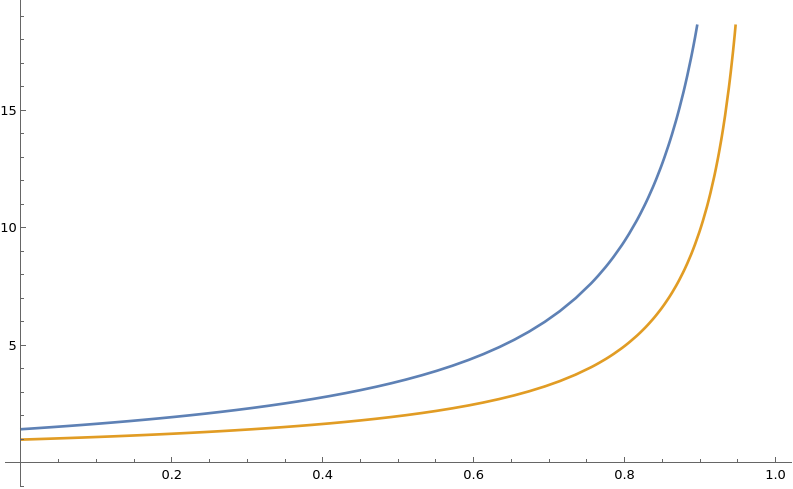
\includegraphics[width=0.75\textwidth]{figures/fig-randomisedwmu}
    \caption{Comparison of the two terms from~\cref{theo:wmu,theo:wmu:rand}: in orange, $\frac{1}{1-\orange{\beta}}$, and in blue, $\frac{1}{\ln\frac{2}{1+\orange{\beta}}}$.}
    \label{fig:mwu:rand:comparison}
\end{figure}
Don't let yourself get fooled by the change of logarithm basis between~\cref{theo:wmu,theo:wmu:rand}: the new bound is always better~--~up to exactly that factor $2$, as $\orange{\beta}\to 1$! (Except, of course, that it is only in expectation).

\begin{framed}
    \noindent\emph{Going further:} for more on this, and connections to online learning and learning theory, see the (excellent) lecture notes by Daniel Hsu, available at \url{https://www.cs.columbia.edu/~djhsu/coms6998-f17/notes.pdf}.
\end{framed}